\documentclass[8pt]{article}
\usepackage{xcolor}
\usepackage{hyperref}
\hypersetup{urlcolor=blue}
\usepackage{times}
\usepackage{pstricks}
\usepackage{listings}
\usepackage{enumerate}
\usepackage{pst-all}
\usepackage{color}
\usepackage{pstcol,pst-node,pst-coil}
\usepackage[dvips]{graphics}
\usepackage{amsfonts,amsmath,amsthm,amssymb,euscript,amscd}
\usepackage[english]{babel}
\usepackage[autostyle]{csquotes}
\usepackage[all,cmtip]{xy}
\usepackage{float}
\usepackage{pdfpages}
\usepackage{graphicx} 
\pagestyle{headings}
\setlength{\parindent}{3ex}
\setlength{\parskip}{1.5ex plus0.5ex minus 0.5ex}
\setlength{\textwidth}{14cm}
\setlength{\oddsidemargin}{1cm}
\setlength{\evensidemargin}{1cm}
\setlength{\textheight}{20.5cm}
\newcommand{\newln}{\\&\quad\quad{}}
\newcommand{\parenthnewln}{\right.\\&\left.\quad\quad{}}
\newcommand{\sub}{\subset} 
\newcommand{\T}{\mathcal{T}}
\newcommand{\R}{\mathbb{R}} 
\newcommand{\U}{\mathcal{U}}
\newcommand{\B}{\mathcal{B}}
\newcommand{\C}{\mathcal{C}}
\newcommand{\8}{\bar}
\newcommand{\maps}{\mapsto}
\newcommand{\norm}[1]{\left\lVert#1\right\rVert}
\newcommand{\e}{\epsilon}
\newcommand{\del}{\delta}
\newcommand{\f}{\frac}
\newcommand{\ol}{\overline}
\newcommand{\la}{\langle}
\newcommand{\ra}{\rangle}
\newcommand{\Par}{\partial}
\renewcommand{\qedsymbol}{\rule{0.7em}{0.7em}}
\newtheorem{theorem}{Theorem}[section]
\newtheorem{lemma}[theorem]{Lemma}
\newtheorem{proposition}[theorem]{Proposition}
\newtheorem{corollary}[theorem]{Corollary}


\begin{document} 
\title{The Science of Decisions} 
\author{\textit{Kris Anaya}}
\date{\today} 
\maketitle

\section{Introduction}
In this task, we are asked to measure the time it takes to name the ink colors in equally-sized lists. In the \textit{congruent} words, the words that are displayed are color words whose names match the colors in which they are printed. In the \textit{incongruent} words conditions, the words displayed are color words whose names do no match the colors in which they are printed.
\subsection{Dependecy} 
Independent variable will be the \textit{congruent} or \textit{incongruent} data sets; whether the font name and colour were smiliar or different. The Depdendent variable will be denoted time $t$ or time between reaction and response. 
\subsection{Hypothesis} 
$H_{0} :=$ \textbf{\textit{there is no difference between \textit{congruent} and \textit{incongruent} population at $\alpha =0.05$}} \newline
$H_{A} :=$ \textbf{\textit{ there are differences between \textit{congruent} and \textit{incongruent} population at $\alpha = 0.05$}} \newline \newline
We will be performing a dependent t-test because we are measuring the same people before and after. Therefore our hypotheses are stated as followed: 
\begin{equation} 
\begin{split} 
H_{0}: \mu_{c} = \mu_{I} \\
H_{A}: \mu_{c} \not= \mu_{I} 
\end{split}
\end{equation} 
\subsection{Statistical test} 
As stated above, we must explore a dependent t-test to ensure that are population difference has relative significance. Secondly, since our sample size is below $30$ and we have an unknown population standard deviation, we shall perform our dependent t-test. We choose dependency because there is one sample that must be tested twice. This test must be a paired test because our patients were tested twice at resulting in different times, thus we measure twice. 
\subsection{Performance} 
\noindent We will perform these task by using a Pythonic language module which we have created. This module is aptly named \textit{statistics.py}. 
The resources for our code may be found within our GitHub page \textit{http://github.com/krismanaya} under \textit{UdactiyDataScience}.  Within our methods, we may conclude that a Type I error is very unlikely. Therefore, the test procedure will be based on a rejection \textbf{$H_{0}$ at an $\alpha$ level of $0.05$}. 
\subsection{Mathematical Variable} 
The given variables  and measures will be the mean, size, standard-error, t-statistics, confidence interval; degrees of freedom, t-critical and Bessel's approximation.These measures and variables will be denoted as:
\begin{center}
\fbox{\parbox{\textwidth}{\textit{Stroop variables:}
\begin{enumerate}
\item $\bar{X}_{c} :=$ \textbf{This mathematical symbol represents the congruent sample mean} 
\item $\bar{X}_{I} :=$ \textbf{This mathematical symbol represents the incongruent sample mean}
\item $\bar{X}_{d} :=$ \textbf{This is the mean difference or $\bar{X}_{I} - \bar{X}_{c}$} 
\item $n_{c,i} := $  \textbf{This mathematical symbol represents the size of the our sample} 
\item $\alpha :=$ \textbf{this symbol represents our alpha level that we are choosing to test}
\item $t_{c} :=$ \textbf{this mathematical symbol represents the critical value of the t score}
\item $t_{stat} :=$ \textbf{this mathematical symbol represents the statistical value of our found t} 
\item $df :=$ \textbf{this is the degrees of freedom or, $t_{n-1}$ score} 
\item $SE :=$ \textbf{this mathematical symbol is the Standard Error} 
\item $\sigma_{c,i} :=$ \textbf{This mathematical symbol is the standard deviation} 
\end{enumerate}}}
\end{center} 
\subsection{Mean/Standard Deviation} 
First, we calculated the mean $\bar{X}_{c,i}$, $\sigma_{c,i}$ and $\bar{X}_{d}$ with help of our functions: 
\begin{table}[htbp]\centering \caption{Stroop statistics \label{sumstat}}
\begin{tabular}{l c c  }\hline\hline
\multicolumn{1}{c}{\textbf{Variable}} & $\bar{X}$ & $\sigma$ \\ \hline
Congruent & 14.05 & 3.56  \\
Incongruent & 22.02 & 4.80  \\
difference & 7.96 & 4.86 \\ 
\multicolumn{1}{c}{n} & \multicolumn{2}{c}{24}\\ \hline
\end{tabular}
\end{table}
\begin{figure}[H]
	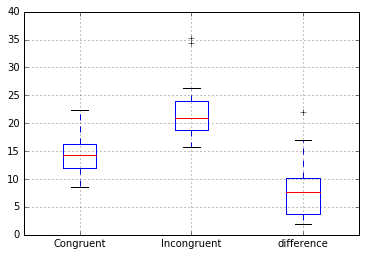
\includegraphics[scale=.5]{box_plot.png}
\end{figure}
Within the table and box plot the reader may observe that the measures, mean and standard deviation reaction time are more improved within the patients \textit{congruent} model then it is for the \textit{incongruent} model. 
\subsection{Dependent t-test} 
Within our central tendencies we wish to calculate the standard error, t-statistic, degrees of freedom and t-critical at $\alpha = 0.05$: 
\begin{table}[htbp]\centering \caption{Stroop statistics \label{sumstat}}
\begin{tabular}{l c c  }\hline\hline
\multicolumn{1}{c}{\textbf{Central Tendencies}}  & $X_{d}$ \\ \hline
$SE$ & 0.99\\
$df$ & 23\\
$t_{stat}$ &  8.020 \\ 
$t_{c}$ &  2.068\\ 
$\alpha$ & 0.05\\
\multicolumn{1}{c}{-} & \multicolumn{2}{c}{-}\\ \hline
\end{tabular}
\end{table}
\begin{figure}[H]
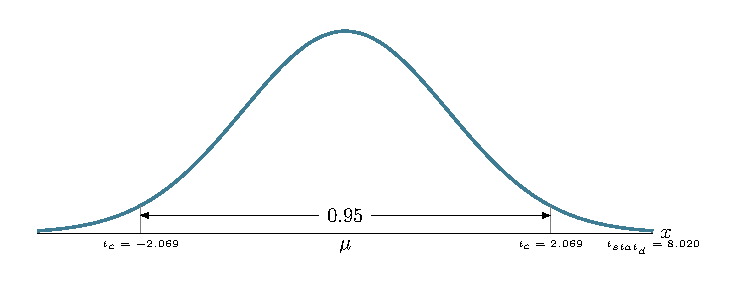
\includegraphics[page=1,scale=0.8]{t_stat_d.pdf} 
\end{figure} 
Here we visualize a t-distribution at $\alpha$ level denoted above and at $0.95$ confidence interval. As we can see our $t_{stat}$ variable is well below the critical value. This suggests that it is possible there is some significant changes between the \textit{congruent} and \textit{incongruent}. Because of this we shall reject $H_{0}$ on both cases where our $t_{stat}$ score falls way below both tails of the critical level. and conclude that there exist a probability $P < \alpha$.
\subsection{Discussion}
The effects responsible for a rejection of $H_{0}$ could be due to the patient's eyes becoming comfortable with words and colors that when they are ready to observe the \textit{incongruent} test their eyes have still not settled. One test you could do is switch the test and perform a Stroop task of \textit{incongruent} then \textit{congruent} and see if the samples differ. Another similar approach for the test would make the patient perform the task multiple times to see if there is some level of improvement after practicing the \textit{incongruent} tests. Finally, a last possibility could be age and eyesight. Do these patients are different in age are they similar? What are the patients eyesight, is it normal or do some patients struggle with color? We do not have more information within the data set.
\end{document}